\section{Aufbau}
\label{sec:Aufbau}

Für den Versuch wird ein koaxialer Germaniumdektektor verwendet. Der Querschnitt des Detektors ist in Abbildung \ref{fig:aufbau} zu sehen.

\begin{figure}[H]
    \centering
    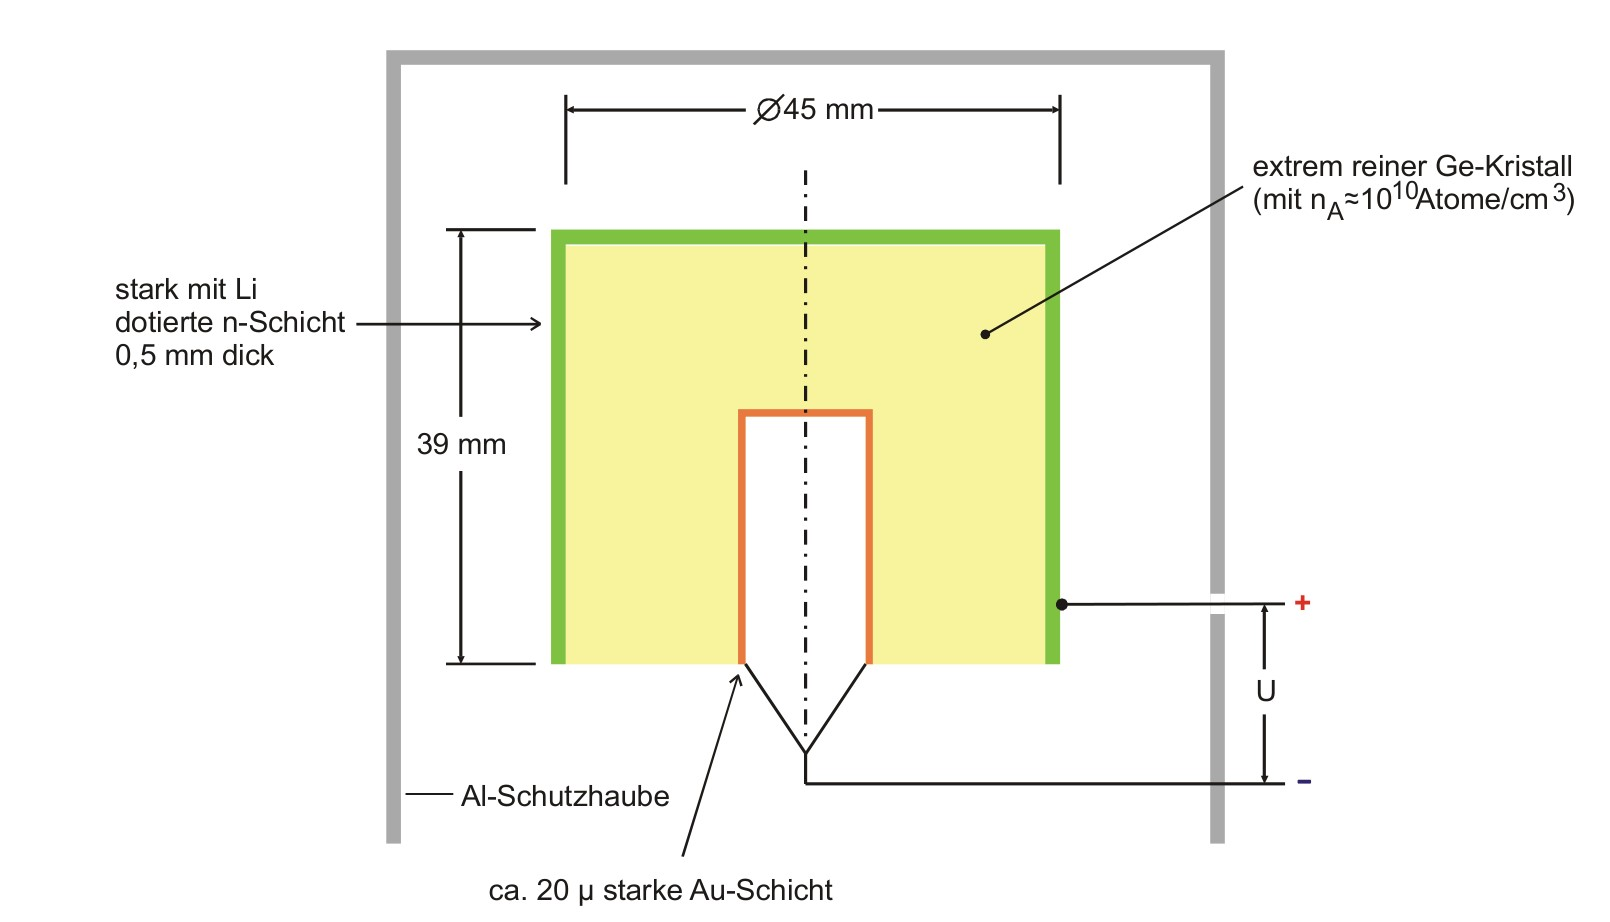
\includegraphics[width=0.8\textwidth]{content/grafik/aufbau.jpg}
    \caption{Der Querschnitt eines koaxialen Germaniumdektektors. \cite{germanium}}
    \label{fig:aufbau}
\end{figure}

Der Detektor ist zylinderförmig und hat einen Durchmesser von $d$ = \qty{45}{\milli\meter} und eine Länge von $l$ = \qty{39}{\milli\meter}.
Um den Ge-Detektor herum befindet sich eine Aluminium Haube, welche zur thermischen und 
elektrischen Isolierung dient. Die Gammaquanten müssen diese Haube durchdringen.
Der gesamte Aufbau ist von einem Blei Kasten umgeben.
Die Quellen der radioaktiven Proben werden mittels eines Abstandshalters, welcher \qty{7}{\centi\meter} lang ist, eingebaut.
Zusätzlich muss beachtet werden, dass der Abstand vom Detektor und der Aluminium
Schutzhaube \qty{1.5}{\centi\meter} beträgt.
